\chapter{Introduzione Generale}
\begin{figure}[!th]
\begin{center}
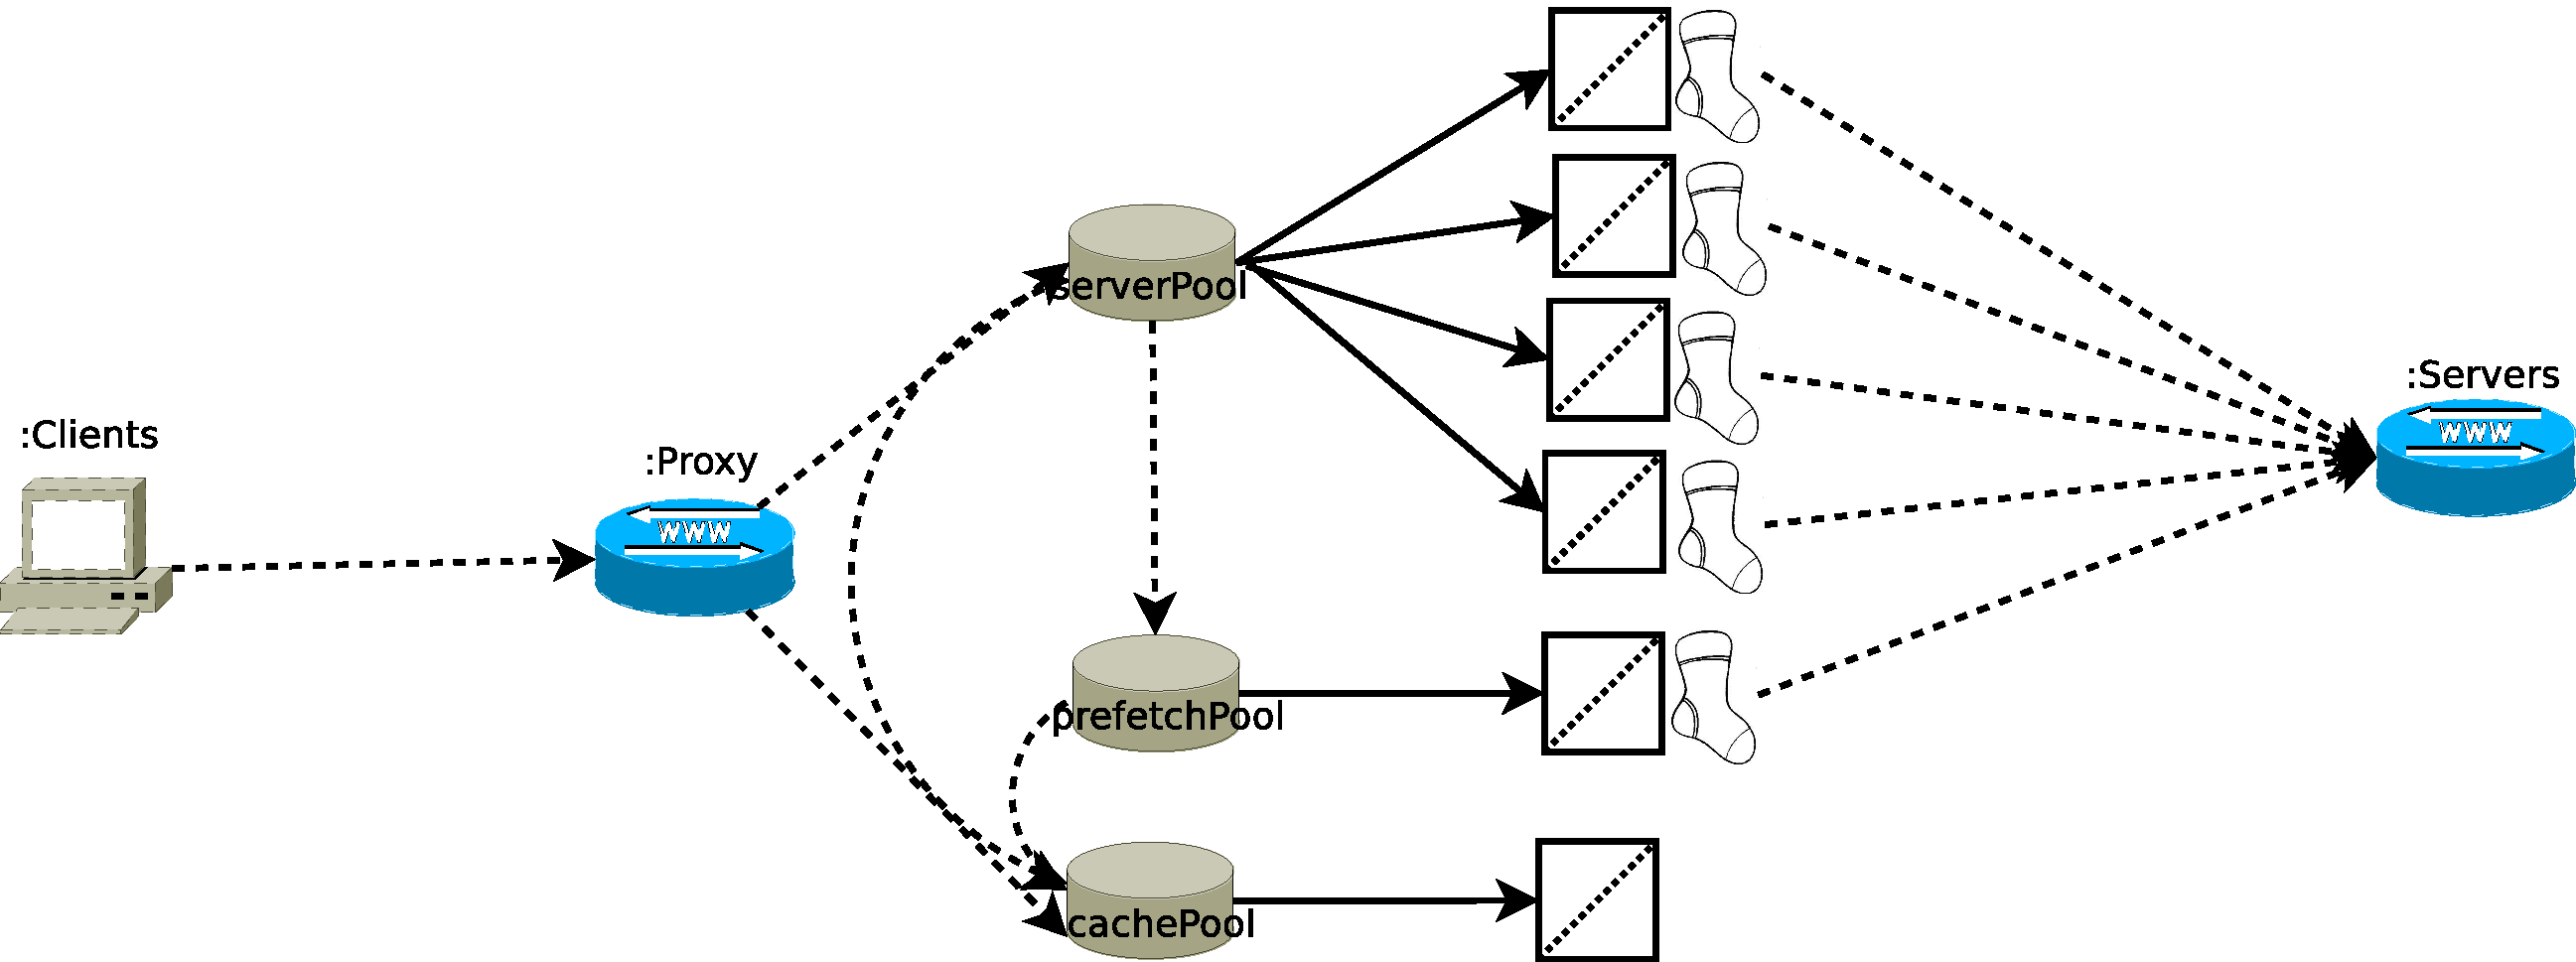
\includegraphics[scale=0.4]{fig/fig02.pdf}
\caption{\textit{Schematizzazione del meccsnismo di comunicazione Client-Proxy-Server,
e rappresentazione ad alto livello dell'architettura del proxy. La semantica di tale
rappresentazione è presente in Figura \vref{fig:gdppw}.}.}
\end{center}
\end{figure}
Con questa relazione, presentiamo il progetto di Redi di Calcolatori per l'Anno
Accademico 2010-2011. Presentiamo la prima versione del proxy, con la quale
abbiamo implementato il prefetch su \textit{N} possibili livelli, con cache 
implementata tramite file-system.

In questo progetto, abbiamo effettuato una gestione delle richieste tramite una
Pool, intesa come ``serbatoio'' di richieste (che è implementata tramite una lista
monodirezionale con sentinella), che può essere utilizzata parametricamente
per ogni tipo di richieste che possono essere gestite dai thread gestori, che possono
essere utilizzati. Si sono utilizzate queste pool anche allo scopo di evitare il
tempo di interleaving dovuti alla presenza di un numero eccessivo di thread
all'interno del sistema proxy, ed il tempo della inizializzazione o distruzione
delle strutture dati associate all'interno della libreria \texttt{pthread}.
Per maggiori dettagli, si veda la Sezione ~\vref{sec:gdp}.

Essendo la cache gestita tramite filesystem, si è rilevato necessario utilizzare
una forma di mutua esclusione per effettuare l'accesso alle risorse presenti
all'interno della cache su file tramite un meccanismo di hashing: questo permette 
appunto di effettuare un locking solamente su di una porzione della memoria (ovvero,
per tutti gli URL di accesso remoto alla risorsa che collidono con lo stesso
numero di hashing), e non sull'intero filesystem. Per maggiori dettagli, si
veda il Capitolo ~\vref{cha:lht}.

Sottolineiamo inoltre che la gestione della connessione avviene tramite un numero
prefissato di tentativi: se una delle operazione causa l'esaurimento di tutti 
i tentativi a disposizione, viene effettuato comunque un tentativo di accesso
in cache in modo da verificare se la risorsa sia eventualmente a disposizione,
altrimenti la comunicazione viene terminata definitivamente.

\section{Compilazione della guida}
La guida è presente sia in questa versione, editata tramite \LaTeX, oppure
tramite \textbf{Doxygen}: per effettuare quest'ultimo tipo di guida, è necessario
disporre di \texttt{graphviz} e \texttt{latex}. Tuttavia, il progetto viene corredato
di tutte le guide già compilate.

\section{Compilazione del progetto}
Il progetto include anche la libreria \texttt{hashtable} di nostra fattura, con la 
quale abbiamo gestito il locking sui file della cache. Non sono pertanto richieste 
librerie aggiuntive fuorchè la \texttt{libpthread}. Il progetto principale 
ha il \texttt{main} contenuto all'interno di \texttt{init.c}. Sono implementate le 
seguenti possibilità:
\begin{description}
\item[\texttt{make clean}:] Pulisce sia il progetto, sia la libreria.
\item[\texttt{make}:] Effettua la compilazione in \textit{ANSI C}.
\item[\texttt{make debug}:] Effettua la compliazione per il debugging.
\end{description}


\section{Esecuzione del progetto}
Eseguendo il progetto con il comando \texttt{proxy --help}, si ottengono le seguenti
informazioni:
\begin{itemize}
\item Tramite il parametro \texttt{-N} o \texttt{-}\texttt{-tree}, si imposta il livello di
	profondità richiesto per effettuare il prefetch delle risorse
\item Tramite il parametro \texttt{-p} o \texttt{-}\texttt{-port}, si imposta la well-known-port
	per il proxy
\item Tramite il parametro \texttt{-i} o \texttt{-}\texttt{-ip}, si imposta l'indirizzo IP verso
	il quale effettuare la ricezione delle richieste sulla well-known-port.
\end{itemize}
